% ------------------------------------------------------------------
%  Calendrier mensuel en grille "Surf & Armorique" - A4 portrait
%  Semaines en lignes, jours en colonnes (lundi -> dimanche).
%  Équivalent stylé du calendrier cal-tex.el (aug24.tex).
%  Compiler avec : pdflatex agenda_mois_grille.tex
%
%  Pour changer de mois, modifier les lignes ci-dessous :
%    \moisnom    : texte affiché dans l'en-tête
%    \firstwd    : jour de la semaine du 1er du mois (1=lundi ... 7=dimanche)
%    \ndays      : nombre de jours du mois (28 à 31)
%    \firstweek  : n° de semaine ISO de la semaine contenant le 1er du mois
%  Options (compteur "jour de l'année / jours restants" comme cal-tex) :
%    \firstdoy   : n° du 1er du mois dans l'année (1er nov. 2026 = 305)
%    \yeardays   : 365 ou 366
%    \isoweeks   : nombre de semaines ISO de l'année (52 ou 53)
%    \showdoytrue / \showdoyfalse pour afficher ou non ce compteur
%    \showampmtrue / \showampmfalse pour les étiquettes AM / PM
%  Chaque case est coupée en deux teintes : matin (haut, plus clair) et après-midi (bas).
% ------------------------------------------------------------------
\documentclass[a4paper]{article}

\usepackage[T1]{fontenc}
\usepackage[utf8]{inputenc}
\usepackage{helvet}
\renewcommand{\familydefault}{\sfdefault}
\usepackage{xcolor}
\usepackage{tikz}
\usepackage[a4paper,left=1cm,right=1cm,top=1.2cm,bottom=1.2cm]{geometry}

\pagestyle{empty}
\setlength{\parindent}{0pt}
\setlength{\parskip}{0pt}

% --- Paramètres du mois --------------------------------------------
\newcommand{\moisnom}{NOVEMBRE 2026}
\newcommand{\firstwd}{7}      % 1er novembre 2026 = dimanche
\newcommand{\ndays}{30}
\newcommand{\firstweek}{44}   % semaine ISO du lundi 26 octobre 2026

% --- Options ---------------------------------------------------------
\newif\ifshowdoy
\showdoytrue
\newcommand{\firstdoy}{305}
\newcommand{\yeardays}{365}
\newcommand{\isoweeks}{53}

% Étiquettes AM / PM dans chaque case (\showampmfalse pour les masquer)
\newif\ifshowampm
\showampmtrue

% --- Couleurs ------------------------------------------------------
\definecolor{gold}{RGB}{209,163,78}
\definecolor{navy}{RGB}{40,52,105}
\definecolor{cream}{RGB}{244,233,207}
\definecolor{paper}{RGB}{252,251,246}
\definecolor{gridgray}{RGB}{160,160,150}
\definecolor{offmonth}{RGB}{236,235,229}
% Teintes de l'après-midi (un cran plus soutenu que le matin)
\definecolor{pmpaper}{RGB}{245,240,226}
\definecolor{pmcream}{RGB}{235,219,186}
\definecolor{pmoff}{RGB}{225,224,216}

% --- Noms des jours (0 = lundi ... 6 = dimanche) --------------------
\newcommand{\wdEN}[1]{\ifcase#1 MONDAY\or TUESDAY\or WEDNESDAY\or THURSDAY\or FRIDAY\or SATURDAY\or SUNDAY\fi}
\newcommand{\wdFR}[1]{\ifcase#1 LUNDI\or MARDI\or MERCREDI\or JEUDI\or VENDREDI\or SAMEDI\or DIMANCHE\fi}

\begin{document}
\noindent\makebox[0pt][l]{%
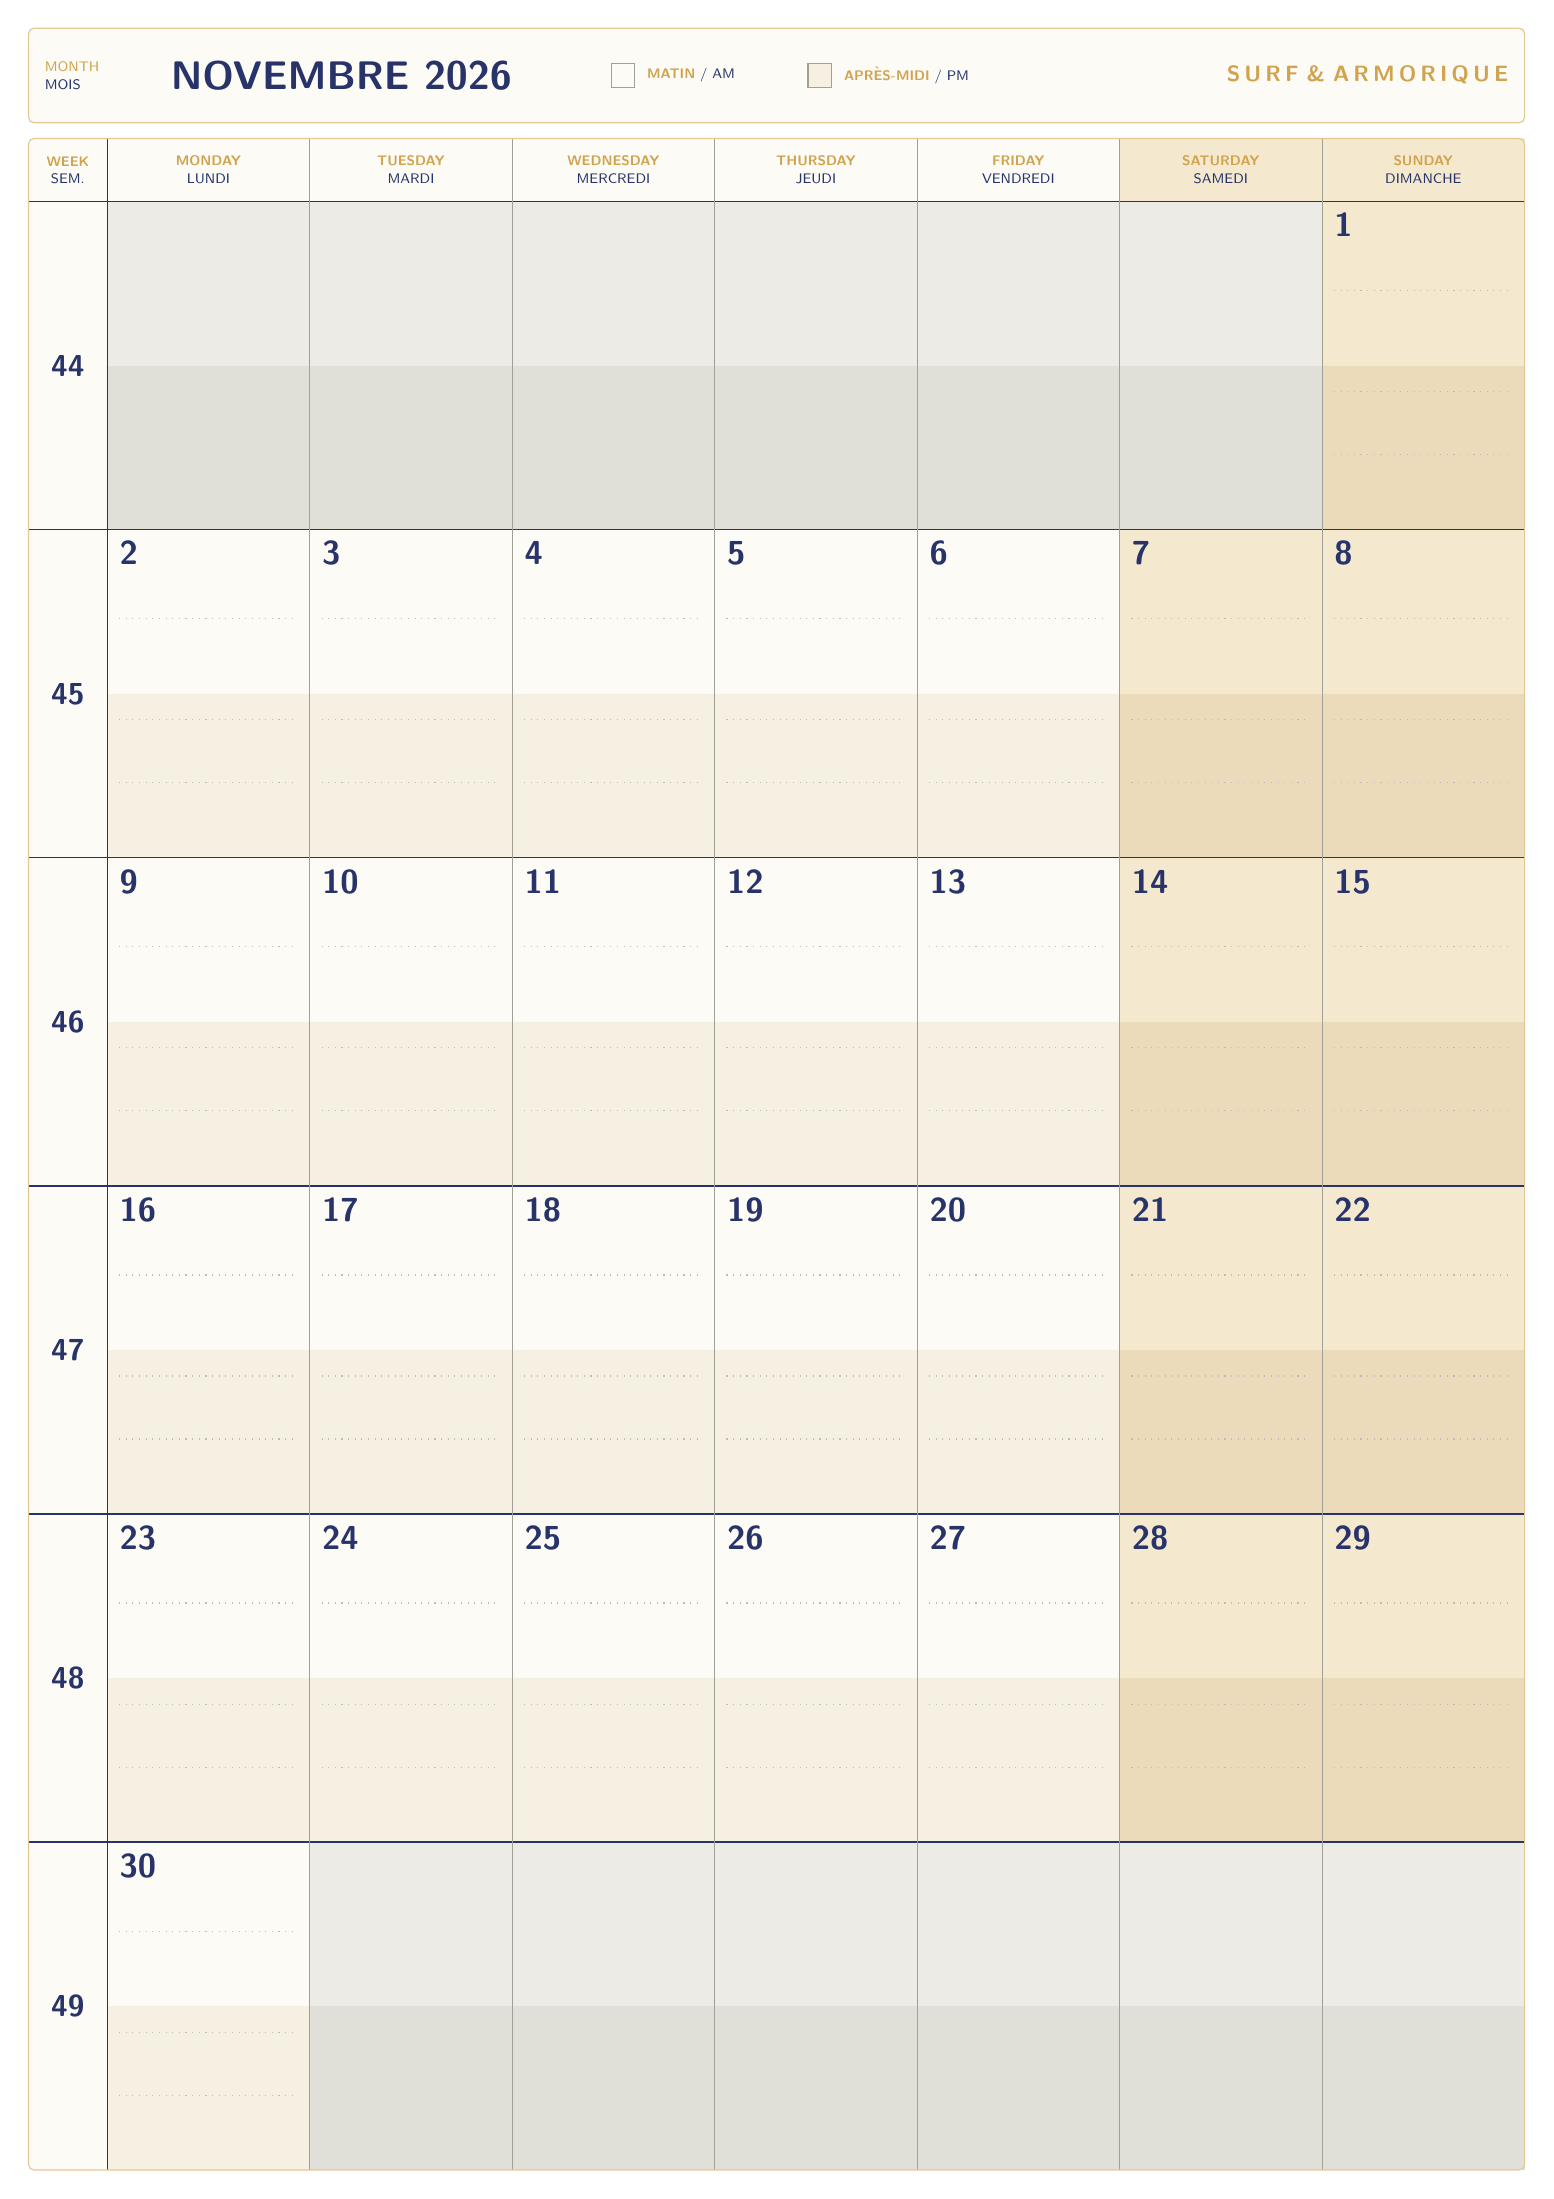
\begin{tikzpicture}[x=1cm,y=1cm]
  % --- Dimensions ---
  \def\PageW{19}
  \def\PageH{27.2}
  \def\hdr{1.2}                          % bandeau d'en-tête
  \def\gap{0.2}                          % espace entre bandeau et grille
  \def\dnb{0.8}                          % hauteur de la ligne des noms de jours
  \def\wkw{1.0}                          % largeur de la colonne des semaines
  \pgfmathsetmacro{\dw}{(\PageW-\wkw)/7}             % largeur d'une colonne-jour
  \pgfmathsetmacro{\yg}{-\hdr-\gap}                  % haut du tableau
  \pgfmathsetmacro{\yr}{\yg-\dnb}                    % haut de la première semaine

  % --- Découpage en semaines (lundi -> dimanche) ---
  \pgfmathtruncatemacro{\lead}{\firstwd-1}
  \pgfmathtruncatemacro{\weeks}{ceil((\lead+\ndays)/7)}
  \pgfmathtruncatemacro{\lastcell}{7*\weeks-1}
  \pgfmathtruncatemacro{\lastrow}{\weeks-1}
  \pgfmathsetmacro{\rh}{(\PageH+\yr)/\weeks}         % hauteur d'une semaine
  \pgfmathsetmacro{\hh}{\rh/2}                       % hauteur matin / après-midi
  \pgfmathtruncatemacro{\nlA}{floor((\hh-0.75)/0.8)}  % lignes d'écriture le matin
  \pgfmathtruncatemacro{\nlP}{floor((\hh-0.25)/0.8)}  % lignes d'écriture l'après-midi

  % --- Bandeau d'en-tête ---
  \fill[paper] (0,0) rectangle (\PageW,-\hdr);
  \draw[gold!60,line width=0.4pt,rounded corners=2pt] (0,0) rectangle (\PageW,-\hdr);
  \node[anchor=west,align=left,inner sep=0,font=\fontsize{5.5}{6.5}\selectfont]
    at (0.2,-0.6) {\textcolor{gold}{MONTH}\\\textcolor{navy}{MOIS}};
  \node[anchor=west,inner sep=0,font=\fontsize{14}{16}\selectfont\bfseries,text=navy]
    at (1.8,-0.6) {\moisnom};
  % légende des teintes
  \draw[gridgray,line width=0.4pt,fill=paper]  (7.4,-0.45) rectangle (7.7,-0.75);
  \node[anchor=west,inner sep=0,font=\fontsize{4.5}{5.5}\selectfont,text=navy] at (7.85,-0.6) {\textcolor{gold}{\bfseries MATIN} / AM};
  \draw[gridgray,line width=0.4pt,fill=pmpaper] (9.9,-0.45) rectangle (10.2,-0.75);
  \node[anchor=west,inner sep=0,font=\fontsize{4.5}{5.5}\selectfont,text=navy] at (10.35,-0.6) {\textcolor{gold}{\bfseries APRÈS-MIDI} / PM};
  \node[anchor=east,inner sep=0,font=\fontsize{8}{9}\selectfont\bfseries,text=gold]
    at ({\PageW-0.2},-0.6) {S\,U\,R\,F\ \textbf{\&}\ A\,R\,M\,O\,R\,I\,Q\,U\,E};

  % --- Fond du tableau ---
  \fill[paper] (0,\yg) rectangle (\PageW,-\PageH);
  % chaque case : moitié haute = matin, moitié basse = après-midi
  \foreach \cellN in {0,...,\lastcell}{%
    \pgfmathtruncatemacro{\col}{mod(\cellN,7)}
    \pgfmathtruncatemacro{\row}{int(\cellN/7)}
    \pgfmathtruncatemacro{\dayD}{\cellN-\lead+1}
    \pgfmathtruncatemacro{\valid}{(\dayD>=1 && \dayD<=\ndays) ? 1 : 0}
    \pgfmathsetmacro{\xl}{\wkw+\col*\dw}
    \pgfmathsetmacro{\yt}{\yr-\row*\rh}
    \pgfmathsetmacro{\ym}{\yr-(\row+0.5)*\rh}
    \pgfmathsetmacro{\yb}{\yr-(\row+1)*\rh}
    \ifnum\valid=0
      \def\tA{offmonth}\def\tP{pmoff}
    \else
      \ifnum\col>4 \def\tA{cream}\def\tP{pmcream}\else \def\tA{paper}\def\tP{pmpaper}\fi
    \fi
    \fill[\tA] (\xl,\yt) rectangle ({\xl+\dw},\ym);
    \fill[\tP] (\xl,\ym) rectangle ({\xl+\dw},\yb);
  }
  % la colonne des semaines reste neutre ; l'en-tête des jours aussi
  \foreach \c in {5,6}{%
    \fill[cream] ({\wkw+\c*\dw},\yg) rectangle ({\wkw+(\c+1)*\dw},\yr);
  }

  % --- Colonne des semaines + ligne des noms de jours ---
  \draw[navy,line width=0.5pt] (0,\yr) -- (\PageW,\yr);
  \draw[navy,line width=0.5pt] (\wkw,\yg) -- (\wkw,-\PageH);
  \node[align=center,inner sep=0,font=\fontsize{5}{6}\selectfont]
    at ({\wkw/2},{\yg-\dnb/2}) {\textcolor{gold}{\bfseries WEEK}\\\textcolor{navy}{SEM.}};
  \foreach \c in {0,...,6}{%
    \node[align=center,inner sep=0,font=\fontsize{5.5}{6.5}\selectfont]
      at ({\wkw+(\c+0.5)*\dw},{\yg-\dnb/2}) {\textcolor{gold}{\bfseries\wdEN{\c}}\\\textcolor{navy}{\wdFR{\c}}};
  }
  \foreach \r in {0,...,\lastrow}{%
    \pgfmathtruncatemacro{\wnum}{mod(\firstweek+\r-1,\isoweeks)+1}
    \node[inner sep=0,font=\fontsize{11}{12}\selectfont\bfseries,text=navy]
      at ({\wkw/2},{\yr-(\r+0.5)*\rh}) {\wnum};
  }

  % --- Lignes de la grille ---
  \foreach \r in {1,...,\lastrow}{%
    \draw[navy,line width=0.6pt] (0,{\yr-\r*\rh}) -- (\PageW,{\yr-\r*\rh});
  }
  \foreach \c in {1,...,6}{%
    \draw[gridgray,line width=0.4pt] ({\wkw+\c*\dw},\yg) -- ({\wkw+\c*\dw},-\PageH);
  }

  % --- Contenu des cases ---
  \foreach \cellN in {0,...,\lastcell}{%
    \pgfmathtruncatemacro{\col}{mod(\cellN,7)}
    \pgfmathtruncatemacro{\row}{int(\cellN/7)}
    \pgfmathtruncatemacro{\dayD}{\cellN-\lead+1}
    \pgfmathtruncatemacro{\valid}{(\dayD>=1 && \dayD<=\ndays) ? 1 : 0}
    \pgfmathsetmacro{\xl}{\wkw+\col*\dw}
    \pgfmathsetmacro{\yt}{\yr-\row*\rh}
    \pgfmathsetmacro{\yb}{\yr-(\row+1)*\rh}
    \ifnum\valid=1
      \node[anchor=north west,inner sep=0,font=\fontsize{12}{13}\selectfont\bfseries,text=navy]
        at ({\xl+0.15},{\yt-0.15}) {\dayD};
      \pgfmathsetmacro{\ym}{\yb+\rh/2}
      \foreach \k in {1,...,\nlA}{%
        \draw[gridgray!70,dotted,line width=0.4pt]
          ({\xl+0.15},{\ym+0.15+\k*0.8}) -- ({\xl+\dw-0.15},{\ym+0.15+\k*0.8});
      }
      \foreach \k in {1,...,\nlP}{%
        \draw[gridgray!70,dotted,line width=0.4pt]
          ({\xl+0.15},{\yb+0.15+\k*0.8}) -- ({\xl+\dw-0.15},{\yb+0.15+\k*0.8});
      }
      \ifshowampm
        \node[anchor=north east,inner sep=0,font=\fontsize{4}{5}\selectfont\bfseries,text=gold]
          at ({\xl+\dw-0.08},{\yt-0.08}) {AM};
        \node[anchor=north east,inner sep=0,font=\fontsize{4}{5}\selectfont\bfseries,text=gold]
          at ({\xl+\dw-0.08},{\ym-0.08}) {PM};
      \fi
      \ifshowdoy
        \pgfmathtruncatemacro{\doy}{\firstdoy+\dayD-1}
        \pgfmathtruncatemacro{\doyrem}{\yeardays-\doy}
        \node[anchor=south east,inner sep=0,font=\fontsize{4.5}{5}\selectfont,text=gridgray]
          at ({\xl+\dw-0.1},{\yb+0.08}) {\doy/\doyrem};
      \fi
    \fi
  }

  % --- Contour du tableau ---
  \draw[gold!60,line width=0.4pt,rounded corners=2pt] (0,\yg) rectangle (\PageW,-\PageH);
\end{tikzpicture}}\par
\end{document}
